\chapter{Ballot design and voting}

This chapter will will describe both the ballot design as well as the voting
process from the perspective of the voter.

\section{Ballot design}

A punchscan ballot consists of two pages stacked atop each other, shown in
figure \ref{fig:punchscan_ballot}. It is uniquely identified by a numerical ID,
printed on both pages. The top page contains the question asked as well as all
possible answers, with each answer being mapped to a symbol --- in this case
the letters `a', `b' and `c'. The bottom page contains the same symbols, which
can be seen through cutouts in the top page when stacked atop each other. Both
the mapping of answers to symbols on the top page, as well as the order of
symbols on the bottom page, are independent random permutations per ballot.

\begin{figure}
\centering
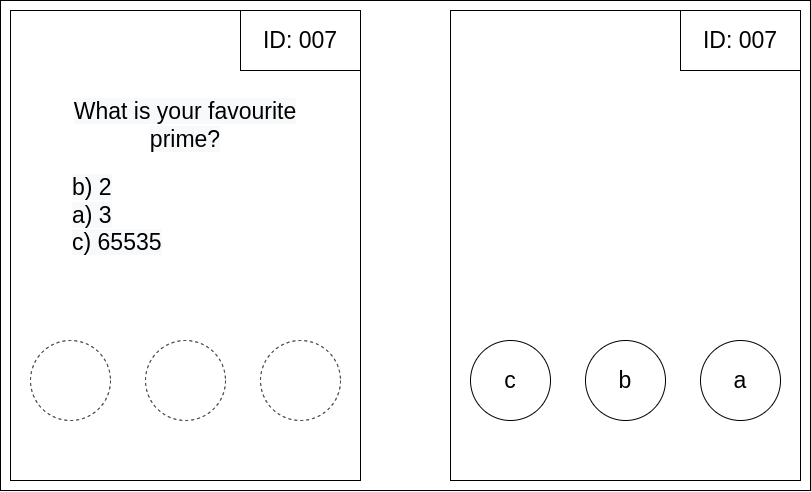
\includegraphics[width=0.8\textwidth]{../resources/high_level_ballot.drawio}
\caption{Punchscan ballot consisting of top (left) and bottom (right) page}
\label{fig:punchscan_ballot}
\end{figure}

\section{Voting process}

After having identified themselves at the polling place, a voter will have to
commit to getting to keep either the top or the bottom page of the ballot as a
receipt. They will then receive a random ballot, consisting of a top and bottom
page stuck together. The voter will read the question and decide on their
answer, and then look for the symbol corresponding to their answer through the
holes in the top page. They will mark their answer using a dauber --- a huge
highlighter as used in Bingo --- thereby leaving a stain on both the top as
well as the bottom page of the ballot. The effect of having marked their choice
is shown in figure \ref{fig:punchscan_ballot_voted}.

The voter will then destroy the page they did not intend to keep by feeding it
through a shredder. The remaining page is scanned by a poll worker. The voter
gets to see and confirm that the scanned page, including an automatic
evaluation of which field was selected, matches their choice. If they agree
with the shown choice, they get to leave, keeping the scanned half of their
ballot as a receipt.

\begin{figure}
\centering
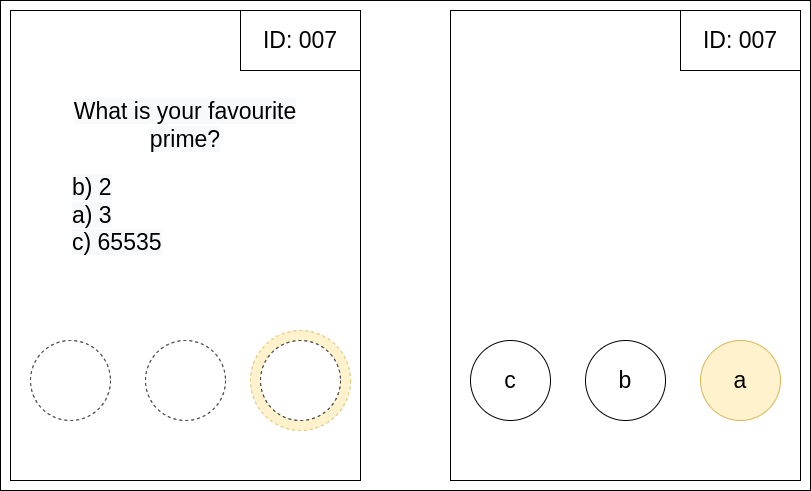
\includegraphics[width=0.8\textwidth]{../resources/high_level_ballot_voted_split.drawio}
\caption{Top (left) and bottom (right) pages of ballot after voter marked their choice}
\label{fig:punchscan_ballot_voted}
\end{figure}
